\section{Material of the earlier evaluation}\label{app:online}

\subsection{Examples}\label{app:examples}
In 2020, Amazon's revenue over the next eight quarters averaged \ExAmznRev{} above its trailing level; the 16-quarter margin implied cumulative operating cash flow of \ExAmznRule{} of trailing revenue, the simulator \ExAmznTwin, and the company reported \ExAmznReal. For General Electric in 2016 (margin \ExGeRule, simulator \ExGeTwin, realized \ExGeReal) and for Ford and General Motors in 2020 the simulator moved away from the realized value: revenue changes of \ExFordRev{} and \ExGmRev{} made it predict \ExFordTwin{} and \ExGmTwin{}, while the companies reported \ExFordReal{} and \ExGmReal{} (margin: \ExFordRule, \ExGmRule). Their consolidated cash flows include captive finance operations that a revenue-driven model does not represent. Among firm-years of firms with more than \$2 billion of revenue and departures larger than 8 points, the simulator's departure has the sign of the realized one \ExRightSign{} of the time.

\subsection{Sensitivity to assumed parameters}
Several parameters are judgment calls rather than estimates: the credit line assumed when none is tagged, the prior on the fixed-cost share and its weight, the shrinkage of trend growth and cyclicality, the coverage thresholds of the market-access cliff, the speed of restructuring and the rating-spread table. Table~\ref{tab:sens} varies each in turn. The incremental correlation against the four-quarter margin ranges from \SensIncrLo{} to \SensIncrHi, and the bankruptcy AUC, on the firm-years of the transmission test, from \SensBkLo{} to \SensBkHi. With a fixed-share prior of 20\% the median error is \SensMaeLow{} points and with 50\% it is \SensMaeHigh. When all eight assumptions vary jointly (a Saltelli design of \SobPoints{} points, each recalibrating the simulator for \SobN{} random firm-years, those of the 320 drawn by the plan that completed every design point; Table~\ref{tab:sobolass}), the median error ranges from \SobMaeMin{} to \SobMaeMax{} and the incremental correlation from \SobIncrMin{} to \SobIncrMax{}. The \SobTopLabel{} alone has a total-effect index of about \SobTopST{} for the error's variance, against \SobRestST{} for all other assumptions together. At the specified values, the same firm-years give a median error of \SobSpecMae{} and an incremental correlation of \SobSpecIncr. Rating spreads come from the version of Damodaran's table published before each cutoff, recovered from the Internet Archive; using the 2026 table instead changes nothing. GDP enters as the vintage published on each cutoff.

\begin{table}[!htbp]
\centering\footnotesize
\caption{Sensitivity to assumed parameters}
\label{tab:sens}
\resizebox{\linewidth}{!}{%
\begin{tabular}{lrrrrr}
\toprule
 & Median error & \multicolumn{2}{c}{Incremental $\rho$ against} & \multicolumn{2}{c}{Baseline score AUC} \\
\cmidrule(lr){3-4}\cmidrule(lr){5-6}
Assumption & (pp of revenue) & 4q margin & regression & Bankruptcy & Severe burn \\
\midrule
As specified & 8.1 & 0.38 & 0.50 & 0.81 & 0.76 \\
\addlinespace
Credit line 4\% of revenue (untagged) & 8.1 & 0.38 & 0.50 & 0.81 & 0.76 \\
Credit line 15\% of revenue (untagged) & 8.1 & 0.38 & 0.50 & 0.81 & 0.77 \\
Fixed-cost prior 20\% & 8.0 & 0.39 & 0.50 & 0.82 & 0.77 \\
Fixed-cost prior 50\% & 8.2 & 0.38 & 0.49 & 0.81 & 0.76 \\
Prior weight 0.5 (data dominate) & 8.1 & 0.38 & 0.50 & 0.81 & 0.76 \\
Prior weight 8 (prior dominates) & 8.1 & 0.38 & 0.50 & 0.81 & 0.76 \\
No shrinkage of growth and cyclicality & 8.1 & 0.38 & 0.50 & 0.81 & 0.76 \\
Market access cut below 2.5$\times$ / 1.5$\times$ coverage & 8.1 & 0.38 & 0.50 & 0.82 & 0.76 \\
Market access cut below 1.0$\times$ / 0.5$\times$, milder cuts & 8.1 & 0.38 & 0.49 & 0.81 & 0.76 \\
Faster, deeper restructuring & 8.0 & 0.39 & 0.50 & 0.82 & 0.76 \\
January 2026 rating table (as in the product) & 8.1 & 0.38 & 0.50 & 0.81 & 0.76 \\
2026 table rescaled by the cutoff's Baa spread & 8.1 & 0.38 & 0.49 & 0.81 & 0.76 \\
\bottomrule
\end{tabular}}

\end{table}

\begin{table}[!htbp]
\centering\scriptsize
\caption{Global (Sobol) sensitivity of the transmission result to the assumed parameters}
\label{tab:sobolass}
\resizebox{\linewidth}{!}{%
\begin{tabular}{lrrlrr}
\toprule
 & & \multicolumn{2}{c}{Median error} & \multicolumn{2}{c}{Incremental $\rho$} \\
\cmidrule(lr){3-4}\cmidrule(lr){5-6}
Assumption & Range & $S_1$ & $S_T$ [95\% CI] & $S_1$ & $S_T$ \\
\midrule
Fixed-cost prior & 0.02--0.6 & 0.43 & 0.52 [0.27, 0.85] & 0.22 & 0.34 \\
Prior s.d. (tau) & 0.02--0.6 & 0.56 & 0.70 [0.50, 1.00] & 0.79 & 0.79 \\
Credit line when untagged & 0.02--0.2 & 0.00 & 0.00 [0.00, 0.01] & 0.00 & 0.00 \\
Weight on own trend growth & 0--1 & 0.00 & 0.00 [0.00, 0.00] & 0.00 & 0.00 \\
Weight on own GDP beta & 0--1 & 0.00 & 0.00 [0.00, 0.00] & 0.00 & 0.00 \\
Coverage below which access is cut & 1--3 & 0.00 & 0.00 [0.00, 0.01] & 0.00 & 0.00 \\
Restructuring speed & 0--0.1 & 0.02 & 0.02 [0.01, 0.16] & 0.00 & 0.02 \\
Restructuring floor & 0.7--1 & 0.02 & 0.02 [0.01, 0.18] & 0.00 & 0.02 \\
\bottomrule
\end{tabular}}

\par\smallskip
\begin{minipage}{\linewidth}\footnotesize
First-order ($S_1$) and total ($S_T$) Sobol indices of the median absolute error and of the incremental correlation against the four-quarter margin, over a joint uniform design with scrambled sequences; bootstrap CI over the base samples. Indices are truncated to $[0, 1]$ and first-order indices to the total index.
\end{minipage}
\end{table}

\subsection{Four-quarter forecasts and calibration}
For S\&P~500 members (today's, a sample selected on survival, and those of 2020), the simulator's four-quarter predictive distributions of revenue improve on a seasonal random walk by \FcRevRw{} and on exponential smoothing \citep{hyndman2008} by \FcRevEts{} in scaled CRPS ($t$ = \FcRevRwT{} and \FcRevEtsT; Table~\ref{tab:fc}). For cash, both benchmarks are better (\FcCashRw{} and \FcCashEts). Blending the simulator into the random walk for cash, with the weight chosen on earlier origins, \CashHybVerdict{} the rule of the earlier evaluation only trivially: the skill is \CashHybSkill{} (CI \CashHybLo--\CashHybHi).

Raw 90\% intervals are too narrow: they cover \CalRevRaw{} of revenue outcomes and \CalCashRaw{} of cash outcomes. Online conformal rescaling \citep{vovk2005}, using only errors whose target quarter ended at least 90 days before the forecast origin, restores coverage to \CalRevConf{} and \CalCashConf{} on average (Table~\ref{tab:cal}, Figure~\ref{fig:cal}), but not in the stress year: for quarters from 2020Q2 to 2021Q1, conformal revenue intervals cover only \CalRevStress. For cash, the raw intervals do not widen for smaller firms ($t$ = \CalCashWidthSizeT{} for size in a regression of interval width) although their errors are larger ($t$ = \CalCashErrSizeT). Rescaling by size and volatility tercile gives \CalCondCash{} coverage for cash and \CalCondRev{} for revenue, and \CalCondCashOk{} the 85--95\% target in every group for cash; adaptive conformal inference \citep{gibbs2021} reaches \CalAciCash{} and \CalAciRev{} (Table~\ref{tab:cal2}). Neither fixes the regime break: in 2020Q2--2021Q1 revenue coverage is \CalCondRevStress{} and \CalAciRevStress.

\begin{table}[!htbp]
\centering\scriptsize
\setlength{\tabcolsep}{3.5pt}
\begin{threeparttable}
\caption{Four-quarter probabilistic forecasts}
\label{tab:fc}
\begin{tabular}{lrrrrrrrr}
\toprule
 & & & \multicolumn{3}{c}{vs.\ seasonal random walk} & \multicolumn{3}{c}{vs.\ ETS} \\
\cmidrule(lr){4-6}\cmidrule(lr){7-9}
 & Pairs & Firms & Skill & Better & DM $t$ & Skill & Better & DM $t$ \\
\midrule
Revenue & 18{,}768 & 470 & 28\% & 68\% & $-$5.41 & 20\% & 57\% & $-$3.67 \\
Cash and short-term investments & 18{,}792 & 473 & $-$27\% & 46\% & 5.33 & $-$35\% & 42\% & 6.61 \\
\bottomrule
\end{tabular}

\begin{tablenotes}\footnotesize
\item Skill: $1-\overline{\mathrm{CRPS}}_{\text{twin}}/\overline{\mathrm{CRPS}}_{\text{benchmark}}$, CRPS scaled by mean quarterly revenue. Better: share of pairs where the simulator's CRPS is lower. DM $t$: Diebold--Mariano statistic clustered by firm and origin (negative: simulator better).
\end{tablenotes}
\end{threeparttable}
\end{table}

\begin{table}[!htbp]
\centering\scriptsize
\caption{Calibration of 90\% predictive intervals}
\label{tab:cal}
\resizebox{\linewidth}{!}{%
\begin{tabular}{lrrrrrrrr}
\toprule
 & \multicolumn{2}{c}{90\% coverage} & \multicolumn{4}{c}{Conformal 90\% coverage, by} & Below & Mean \\
\cmidrule(lr){2-3}\cmidrule(lr){4-7}
 & Raw & Conformal & Other targets & 2020Q2--2021Q1 & $h$ = 1 / 4 & Small / large firms & 5\% quantile & PIT \\
\midrule
Revenue & 78\% & 91\% & 93\% & 78\% & 91\% / 93\% & 92\% / 90\% & 13\% & 0.47 \\
Cash & 39\% & 91\% & 92\% & 89\% & 93\% / 90\% & 89\% / 95\% & 35\% & 0.44 \\
\bottomrule
\end{tabular}}

\end{table}

\begin{table}[!htbp]
\centering\scriptsize
\caption{Coverage of 90\% intervals with group-conditional and adaptive conformal calibration}
\label{tab:cal2}
\begin{tabular}{lllrr}
\toprule
Variable & Split & Group & Group-conditional & Adaptive (ACI) \\
\midrule
Revenue & Target quarters & 2020Q2-2021Q1 & 79\% & 78\% \\
Revenue & Target quarters & other & 92\% & 93\% \\
Revenue & Size tercile & low & 90\% & 92\% \\
Revenue & Size tercile & mid & 91\% & 90\% \\
Revenue & Size tercile & high & 91\% & 90\% \\
Revenue & Volatility tercile & low & 90\% & 87\% \\
Revenue & Volatility tercile & mid & 91\% & 92\% \\
Revenue & Volatility tercile & high & 90\% & 93\% \\
\addlinespace
Cash & Target quarters & 2020Q2-2021Q1 & 88\% & 89\% \\
Cash & Target quarters & other & 91\% & 92\% \\
Cash & Size tercile & low & 92\% & 89\% \\
Cash & Size tercile & mid & 90\% & 90\% \\
Cash & Size tercile & high & 91\% & 95\% \\
Cash & Volatility tercile & low & 91\% & 89\% \\
Cash & Volatility tercile & mid & 91\% & 92\% \\
Cash & Volatility tercile & high & 91\% & 93\% \\
\bottomrule
\end{tabular}

\end{table}

\begin{figure}[!htbp]
\centering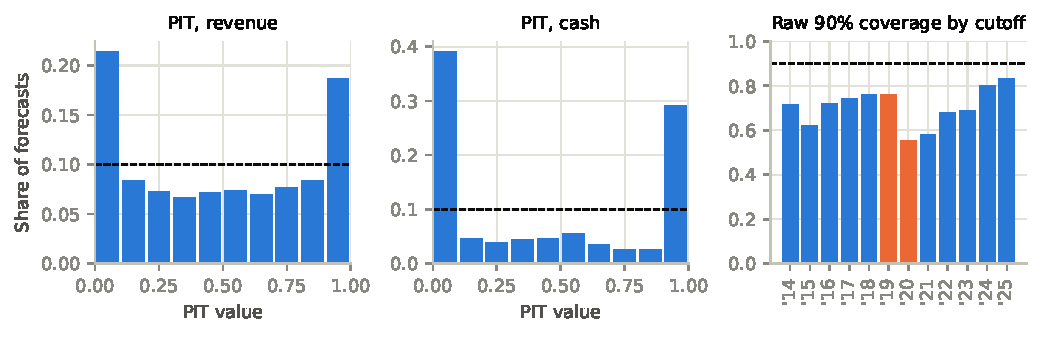
\includegraphics[width=\linewidth]{figures/calibration.pdf}
\caption{Coverage of raw and conformally rescaled 90\% intervals by forecast origin.}
\label{fig:cal}
\end{figure}

\subsection{2020 and two other downturns}
Table~\ref{tab:covid} repeats the 2020 cross-section for the \CovAllN{} filers alive on 20 February 2020 and for the \CovSpN{} members of the S\&P~500 on that date. The simulator's stress score ranks raw cash burn (\CovAllTwin{} in the full sample, \CovSpTwin{} in the S\&P), the FCF margin ranks it better (\CovAllFcf, \CovSpFcf), and no predictor's correlation with abnormal burn exceeds 0.2 in absolute value. Giving each firm the median realized revenue shock of its industry peers (Table~\ref{tab:exposure}; median depth \ExpDepth), the simulator ranks raw burn at \ExpTwinRaw{} against \ExpUniformRaw{} under the uniform freeze; in a rank regression with the FCF margin and the health formula, clustered by industry, its coefficient for abnormal burn has $t$ = \ExpTwinAbnT, and the formula's $t$ = \ExpFormulaAbnT. Table~\ref{tab:episodes} applies the same design to the eight quarters after the 2015, 2020 and 2022 cutoffs (\EpiFifteenClusters--\EpiTwentyTwoClusters{} industry clusters). Because the shocks are realized, these regressions decompose outcomes; they are not forecasts.

\begin{table}[!htbp]
\centering\scriptsize
\caption{2020--21 cash burn, predictors frozen on 20 February 2020}
\label{tab:covid}
\begin{tabular}{lrrrr}
\toprule
 & \multicolumn{2}{c}{All filers ($n$ = 1{,}651)} & \multicolumn{2}{c}{S\&P 500 on 20 Feb 2020 ($n$ = 341)} \\
\cmidrule(lr){2-3}\cmidrule(lr){4-5}
 & Raw burn & Abnormal burn & Raw burn & Abnormal burn \\
\midrule
Twin: stress health score & 0.33 & 0.04 & 0.34 & 0.16 \\
Twin: baseline health score & 0.38 & 0.03 & 0.34 & 0.15 \\
Health formula, no simulation & 0.34 & 0.02 & 0.34 & 0.13 \\
\addlinespace
Altman Z$''$ & 0.28 & 0.02 & 0.37 & 0.11 \\
Ohlson O-score & 0.31 & $-$0.01 & 0.26 & 0.12 \\
Zmijewski score & 0.21 & 0.03 & 0.24 & 0.14 \\
Interest coverage & 0.30 & 0.03 & 0.31 & 0.14 \\
Net debt / EBITDA & 0.26 & $-$0.01 & 0.29 & 0.09 \\
Cash / revenue & 0.19 & 0.04 & 0.44 & 0.06 \\
Current ratio & 0.09 & 0.05 & 0.29 & 0.14 \\
Static stress test & 0.20 & 0.01 & 0.14 & 0.03 \\
Revenue volatility & 0.16 & 0.01 & 0.08 & 0.08 \\
Fixed-cost share & 0.00 & $-$0.02 & $-$0.15 & $-$0.03 \\
Size (log revenue) & 0.14 & $-$0.05 & $-$0.27 & $-$0.09 \\
\addlinespace
Trailing FCF margin & 0.66 & $-$0.14 & 0.83 & 0.09 \\
Capex / revenue & 0.03 & $-$0.04 & 0.11 & 0.13 \\
\bottomrule
\end{tabular}

\par\smallskip
\begin{minipage}{\linewidth}\footnotesize
Spearman correlation between each risk-oriented predictor and realized burn severity. Raw burn: cumulative FCF over the quarters reported between mid-January 2020 and mid-July 2021 as a share of trailing revenue, sign reversed; abnormal burn: the same after subtracting each company's pre-2020 run-rate.
\end{minipage}
\end{table}

\begin{table}[!htbp]
\centering\scriptsize
\caption{Fragility and exposure in 2020}
\label{tab:exposure}
\resizebox{\linewidth}{!}{%
\begin{tabular}{lrrrrrrrr}
\toprule
 & \multicolumn{4}{c}{Spearman $\rho$ with burn} & \multicolumn{4}{c}{Rank regression, coefficient ($t$)} \\
\cmidrule(lr){2-5}\cmidrule(lr){6-9}
Outcome & Twin, uniform freeze & Industry shock alone & Twin at industry shock & FCF margin & Industry shock & Twin at shock & FCF margin & Formula \\
\midrule
Raw burn & 0.33 & 0.11 & 0.37 & 0.66 & 0.07 (3.4) & 0.16 (3.1) & 0.60 (14.1) & $-$0.04 ($-$0.7) \\
Abnormal burn & 0.04 & 0.09 & 0.04 & $-$0.14 & 0.09 (3.5) & 0.14 (1.9) & $-$0.19 ($-$4.0) & $-$0.02 ($-$0.3) \\
\bottomrule
\end{tabular}}

\par\smallskip
\begin{minipage}{\linewidth}\footnotesize
Industry shock: leave-one-out median of peers' worst year-on-year revenue change in 2020--21 (2-digit SIC with at least five peers, else Fama--French industry); realized information, a decomposition. Rank regression: OLS of percentile ranks, $t$-statistics clustered by industry.
\end{minipage}
\end{table}

\begin{table}[!htbp]
\centering\scriptsize
\caption{Fragility given exposure in three downturns}
\label{tab:episodes}
\resizebox{\linewidth}{!}{%
\begin{tabular}{lrrlrrrr}
\toprule
 & & Median & & \multicolumn{4}{c}{Rank regression $t$, industry-clustered} \\
\cmidrule(lr){5-8}
Episode & Firms & shock & Burn & Industry shock & Twin at shock & FCF margin & Formula \\
\midrule
2015--16 commodity bust (cutoff Feb 2015) & 1{,}811 & 9\% & raw & 1.4 & 3.2 & 21.4 & $-$1.8 \\
 &  &  & abnormal & 0.9 & 2.0 & $-$7.4 & $-$1.2 \\
\addlinespace
2020 pandemic (Feb 2020) & 1{,}766 & 18\% & raw & 2.9 & 4.8 & 17.0 & $-$2.7 \\
 &  &  & abnormal & 2.2 & 4.0 & $-$3.7 & $-$1.9 \\
\addlinespace
2022 rate shock (Feb 2022) & 1{,}846 & 8\% & raw & 1.1 & 4.2 & 17.0 & $-$3.8 \\
 &  &  & abnormal & 0.6 & 4.6 & $-$7.2 & $-$3.9 \\
\bottomrule
\end{tabular}}

\par\smallskip
\begin{minipage}{\linewidth}\footnotesize
Rank regression of burn severity over the eight quarters after the cutoff on the percentile ranks of the industry's leave-one-out realized revenue shock, the simulator's stress score at that shock, the trailing FCF margin and the health formula; $t$-statistics clustered by 2-digit SIC industry.
\end{minipage}
\end{table}

\subsection{Implementation}
The Python reference engine (NumPy) performs calibration, experiments and exports. A TypeScript port runs in a Web Worker, so the public dashboard needs no server; golden runs exported from Python with identical pre-drawn shocks must agree to a relative tolerance of $10^{-9}$. The balance-sheet identity is checked by property-based tests, the data pipeline including 52/53-week fiscal calendars is tested end to end on synthetic XBRL, and a synthetic test checks that the transmission statistics reject a predictor that is merely smoother than the base rule. The revision-3 run read the frozen snapshot on x86 servers; each result records the code digest, the lock file (\texttt{\LockDigest}) and the snapshot digest.
